% Provenance (never printed): see sources/outline_sources.md (Year 2: natural hazards and risks
% quantified --- recurrence, probabilistic hazard, slope stability, tsunamis, floods, warning).
% Terminology from the UN report A/71/644 (UNDRR); the 475-year convention from the USGS
% Earthquake Hazards 201 page; the ground-motion prediction equation of Boore, Joyner and Fumal
% (USGS Open-File Report 93-509); run-ups from the NOAA NCEI tsunami database; the 1999 Vargas
% debris flows from USGS Open-File Report 01-0144. Ledger rows in sources/ledger/book4.md;
% curves and numbers from figdata/bachelor-2/hazards.py and the Book 4 second-writer scratch
% calculator calc/ch28.py. Hazards are described and quantified physically only: no advice.
\chapter{Peligros geológicos y riesgo}\label{ch:b2:geological-hazards}

Un edificio diseñado para el movimiento del suelo que se supera, por término medio, una vez cada 475 años tiene una
probabilidad entre diez de sufrirlo durante una vida útil de cincuenta años. Las dos afirmaciones son la misma cifra
leída de dos maneras, y pasar de una a otra es el trabajo diario de la ciencia de los peligros. Este capítulo
construye sus herramientas: la probabilidad de los sucesos raros, la \omterm{def:b2:geological-hazards:psha}{curva de peligrosidad} de un emplazamiento, la estabilidad de un
talud, la velocidad y el \omterm{def:b2:geological-hazards:tsunami}{remonte de un tsunami}, la frecuencia de las crecidas, y la física que determina
con cuánta antelación puede avisarse de cada peligro.
% ledger: usgs:eh201-475

\begin{recall}
\textbf{De los volúmenes escolares}: peligro natural, catástrofe natural y deslizamiento de tierra; vulnerabilidad,
riesgo, prevención y mapa de peligrosidad; tsunami; el \omterm{def:b2:geological-hazards:return}{periodo de retorno} de una crecida, y la fórmula del rango
$T = (n + 1)/m$ para un registro de $n$ caudales máximos anuales. \textbf{Del volumen de primer año}: la
ley de Gutenberg--Richter $\log_{10} N(\geq M) = a - bM$ y su valor b; el momento sísmico y la magnitud
de momento; la presión intersticial, la tensión efectiva $\sigma' = \sigma - u$ y el criterio de rotura de
Coulomb $\tau = c' + \sigma' \tan\varphi'$. \textbf{Del \cref{ch:b2:eruptive-styles}}: las \omterm{def:b2:eruptive-styles:pdc}{corrientes de densidad
piroclásticas}, los \omterm{def:b2:eruptive-styles:lahar}{lahares} y la caída de \omterm{def:b2:eruptive-styles:tephra}{tefra}. \textbf{De los libros de matemáticas}: las distribuciones de Poisson y
exponencial, la distribución normal y su función de distribución $\Phi$.
\textbf{Del volumen de segundo año de los libros de física}: la relación de dispersión de las ondas de gravedad superficiales,
$\omega^2 = gk\tanh(kh)$.
\end{recall}

\section{Peligro, exposición y riesgo}\label{sec:b2:geological-hazards:risk}

\begin{definition}[Peligro geológico, exposición, riesgo de desastre]\label{def:b2:geological-hazards:risk}
Un \emph{peligro geológico}\index{peligro geologico@peligro geológico} es un proceso o fenómeno que se origina en
los procesos internos de la Tierra ---un terremoto, una erupción, un movimiento de masa como un
deslizamiento o un flujo de derrubios--- y que puede causar pérdida de vidas, lesiones, daños o perturbaciones. Se
caracteriza por su localización, su intensidad o magnitud, y su frecuencia o probabilidad. La
\emph{exposición}\index{exposicion (a un peligro)@exposición (a un peligro)} a un peligro es la situación de las personas,
los edificios, las infraestructuras y otros bienes situados donde el peligro puede alcanzarlos, medida por su
número o su valor. El \emph{riesgo de desastre}\index{riesgo de desastre} es la posible pérdida de vidas,
de salud o de bienes que podría producirse en un periodo dado, determinada probabilísticamente a partir del
peligro, la exposición y la vulnerabilidad de lo expuesto.
\end{definition}
% ledger: undrr:hazard, undrr:geological, undrr:exposure, undrr:disaster-risk, undrr:vulnerability

La terminología internacional clasifica aparte los tsunamis: desencadenados por terremotos y otros
sucesos geológicos, se convierten en un proceso oceánico y golpean como un peligro costero, relacionado con el agua.
Este capítulo los trata con los demás, porque su origen es geológico.
% ledger: undrr:geological

La definición contiene un producto. Si los sucesos de intensidad $i$ se producen con una tasa anual
$\lambda_i$, si los bienes expuestos valen $E$ y si un suceso de intensidad $i$ destruye una
fracción $V_i$ de ellos (la vulnerabilidad, entre 0 y 1), la pérdida anual esperada es
\begin{equation}
L = \sum_i \lambda_i \, E \, V_i ,
\label{eq:b2:geological-hazards:loss}
\end{equation}
a menudo abreviada como riesgo = peligro $\times$ \omterm{def:b2:geological-hazards:risk}{exposición} $\times$ vulnerabilidad. El riesgo se anula cuando
se anula cualquier factor: un volcán violento en una isla deshabitada, una ciudad poblada sobre un \omterm{def:b2:precambrian-earth:craton}{cratón} tranquilo, o
unos edificios que resisten la sacudida. La ciencia de los peligros mide el primer factor; la figura siguiente
lo sitúa entre los tres.

\begin{omfigure}
\centering
\begin{tikzpicture}[font=\small]
\fill[omThm!14] (90:1.05) circle (1.55);
\fill[omDef!14] (210:1.05) circle (1.55);
\fill[black!8] (330:1.05) circle (1.55);
\begin{scope}
\clip (90:1.05) circle (1.55);
\clip (210:1.05) circle (1.55);
\fill[omThm!45!omDef!45] (330:1.05) circle (1.55);
\end{scope}
\draw[omThm, thick] (90:1.05) circle (1.55);
\draw[omDef, thick] (210:1.05) circle (1.55);
\draw[black!60, thick] (330:1.05) circle (1.55);
\node[align=center, anchor=south] at (0,2.65) {\textbf{peligro} {\scriptsize (tasa $\lambda_i$, intensidad)}};
\node[align=right, anchor=east] at (-2.55,-1.35) {\textbf{exposición}\\[-1pt]{\scriptsize bienes $E$}};
\node[align=left, anchor=west] at (2.55,-1.35) {\textbf{vulnerabilidad}\\[-1pt]{\scriptsize fracción perdida $V_i$}};
\node[align=center, font=\scriptsize\bfseries] at (0,0) {riesgo};
\end{tikzpicture}
\par\smallskip{\small Los tres factores del \omterm{def:b2:geological-hazards:risk}{riesgo de desastre}. La pérdida esperada solo es distinta de cero donde
se solapan los tres: un peligro que alcanza algo expuesto y susceptible de sufrir daño.}
\end{omfigure}

\section{La probabilidad de los sucesos raros}\label{sec:b2:geological-hazards:probability}

\begin{definition}[Periodo de retorno]\label{def:b2:geological-hazards:return}
Supóngase que sucesos de un tipo dado ---una crecida por encima de un caudal, un movimiento del suelo por encima de un nivel, un
terremoto por encima de una magnitud--- se producen con una tasa anual media $\lambda$. Su \emph{periodo de
retorno}\index{periodo de retorno} es $T = 1/\lambda$: el intervalo medio entre dos de ellos, y la
inversa de su tasa anual, no un calendario.
\end{definition}
% ledger: usgs:eh201-475

\begin{definition}[Probabilidad de excedencia]\label{def:b2:geological-hazards:poisson}
La \emph{probabilidad de excedencia}\index{probabilidad de excedencia} de un nivel en un tiempo de \omterm{def:b2:geological-hazards:risk}{exposición} $t$
es la probabilidad de que el nivel se iguale o se supere al menos una vez durante $t$.
\end{definition}

\begin{proposition}[Modelo de recurrencia de Poisson]\label{prop:b2:geological-hazards:poisson}
Supóngase que los sucesos se producen de uno en uno\index{modelo de recurrencia de Poisson}, con independencia unos de
otros y del tiempo transcurrido, con una tasa media constante $\lambda = 1/T$. Entonces el número $N$ de
sucesos en un tiempo $t$ sigue la distribución de Poisson de media $\lambda t$; la \omterm{def:b2:geological-hazards:poisson}{probabilidad de
excedencia} en $t$ es
\begin{equation}
P(t) = 1 - e^{-t/T};
\label{eq:b2:geological-hazards:poisson}
\end{equation}
y el intervalo entre sucesos consecutivos sigue la distribución exponencial de media $T$.
\end{proposition}

\begin{proof}
Sea $P_k(t)$ la probabilidad de $k$ sucesos en $[0, t]$. En un intervalo corto $\mathrm{d}t$ se
produce un suceso con probabilidad $\lambda\,\mathrm{d}t$, con independencia del pasado, y dos con una
probabilidad de orden superior. Por tanto, $P_0(t + \mathrm{d}t) = P_0(t)(1 - \lambda\,\mathrm{d}t)$, es decir,
$P_0' = -\lambda P_0$ con $P_0(0) = 1$: $P_0(t) = e^{-\lambda t}$, y $P(t) = 1 - P_0(t)$. Del
mismo modo, $P_k' = \lambda(P_{k-1} - P_k)$ para $k \geq 1$, que se resuelve por inducción:
$P_k(t) = (\lambda t)^k e^{-\lambda t}/k!$, la distribución de Poisson de media $\lambda t$. Partiendo de
un suceso, el mismo razonamiento da la probabilidad de que el siguiente llegue después de $t$:
$e^{-\lambda t}$, la función de supervivencia de la distribución exponencial, cuya media es
$\int_0^\infty e^{-\lambda t}\,\mathrm{d}t = 1/\lambda = T$.
\end{proof}

Dos consecuencias se usan en todas partes. Para una probabilidad $p$ en un tiempo de \omterm{def:b2:geological-hazards:risk}{exposición} $t$, el \omterm{def:b2:geological-hazards:return}{periodo
de retorno} es $T = -t/\ln(1 - p)$: un \qty{10}{\percent} en 50 años da $T = 50/0.10536 =
474.6$ años, el movimiento «de 475 años» de las normas de construcción, y un \qty{2}{\percent} en 50 años
da 2475 años. Y cuando $t \ll T$, $P \approx t/T$: la tasa puede leerse como una
probabilidad anual. A lo largo de un \omterm{def:b2:geological-hazards:return}{periodo de retorno} completo, en cambio, la probabilidad es $1 - e^{-1} =
\qty{63}{\percent}$, no 1. La figura siguiente (izquierda) representa \eqref{eq:b2:geological-hazards:poisson}
para tres \omterm{def:b2:geological-hazards:return}{periodos de retorno}.
% ledger: usgs:eh201-475
% values: T 474.561 and 2474.92 years; P(50|475) 0.0999 (hazards.py numbers)

¿Es cierto el modelo? El catálogo mundial de terremotos de magnitud igual o superior a 7 contiene 696 sucesos
de 1976 a 2025, 695 intervalos con una media de 26.2 días. Si fueran un proceso de Poisson,
la fracción de intervalos más largos que $t$ sería $e^{-t/26.2}$, una recta en un eje
logarítmico. La figura siguiente (derecha) muestra que casi lo es: el \qty{30.4}{\percent} de los intervalos es
más largo que 30 días, frente al \qty{31.8}{\percent} del modelo, y la desviación típica de los
intervalos es 1.07 veces su media, frente a exactamente 1. El defecto está en los intervalos cortos: 36 pares
caen el mismo día, réplicas y dobletes que un proceso sin memoria no agruparía. Por eso los mapas de
peligrosidad eliminan de un catálogo los sucesos dependientes, lo desagrupan, de modo que los
terremotos principales restantes puedan tratarse como un proceso de Poisson; sus tasas por magnitud proceden de la
ley de Gutenberg--Richter.
% ledger: data:usgs-comcat, usgs:eh201-poisson
% values: m7_events 696, mean 26.2245 d, cv 1.06891, same-day 36, frac>30 d 0.303597 vs 0.318552

\begin{omfigure}
\centering
\begin{minipage}[b]{0.49\linewidth}\centering
\begin{tikzpicture}
\begin{axis}[omrecord, width=0.96\linewidth, height=5.2cm, xmin=0, xmax=200, ymin=0, ymax=1,
  xlabel={tiempo de exposición $t$ (años)}, ylabel={probabilidad de excedencia},
  tick label style={font=\scriptsize}, label style={font=\small},
  xtick={0,50,100,150,200}, ytick={0,0.2,...,1}]
% computed in figdata/bachelor-2/hazards.py part poisson
\addplot[omThm, line width=1pt] table[x=t_yr, y=P50] {figdata/out/bachelor-2-hazards-poisson.dat};
\addplot[omDef, line width=1pt] table[x=t_yr, y=P475] {figdata/out/bachelor-2-hazards-poisson.dat};
\addplot[black!70, line width=1pt, densely dashed] table[x=t_yr, y=P2475] {figdata/out/bachelor-2-hazards-poisson.dat};
\draw[black!50, densely dotted] (axis cs:50,0) -- (axis cs:50,1);
\fill[omDef] (axis cs:50,0.1) circle (1.8pt);
\node[font=\scriptsize, text=omThm, anchor=west] at (axis cs:62,0.86) {$T = 50$};
\node[font=\scriptsize, text=omDef, anchor=west] at (axis cs:120,0.34) {$T = 475$};
\node[font=\scriptsize, text=black!70, anchor=west] at (axis cs:120,0.12) {$T = 2475$};
\node[font=\scriptsize, anchor=west, text=omDef] at (axis cs:52,0.2) {\qty{10}{\percent}};
\end{axis}
\end{tikzpicture}
\end{minipage}\hfill
\begin{minipage}[b]{0.49\linewidth}\centering
\begin{tikzpicture}
\begin{axis}[omrecord, width=0.93\linewidth, height=5.2cm, xmin=0, xmax=120, ymode=log,
  ymin=0.008, ymax=1.1, xlabel={intervalo $t$ (días)}, ylabel={fracción de intervalos $> t$},
  tick label style={font=\scriptsize}, label style={font=\small}, xtick={0,30,60,90,120},
  legend style={at={(0.03,0.03)}, anchor=south west, font=\scriptsize, draw=black!30},
  legend cell align=left]
% computed in figdata/bachelor-2/hazards.py part survival; ledger: data:usgs-comcat
\addplot[omThm, only marks, mark=*, mark size=1.2pt] table[x=t_day, y=observed] {figdata/out/bachelor-2-hazards-survival.dat};
\addlegendentry{$M \geq 7$, 1976--2025}
\addplot[black, line width=0.9pt] table[x=t_day, y=poisson] {figdata/out/bachelor-2-hazards-survival.dat};
\addlegendentry{Poisson, media 26.2 días}
\end{axis}
\end{tikzpicture}
\end{minipage}
\par\smallskip{\small Izquierda: la probabilidad de al menos un suceso en un tiempo de \omterm{def:b2:geological-hazards:risk}{exposición} $t$ para
\omterm{def:b2:geological-hazards:return}{periodos de retorno} de 50, 475 y 2475 años; el suceso de 475 años tiene una probabilidad del \qty{10}{\percent} en 50
años. Derecha: los intervalos entre los 696 terremotos de magnitud igual o superior a 7 del catálogo
mundial de 1976--2025, frente a la ley exponencial de un proceso de Poisson de la misma tasa. Datos:
USGS ANSS Comprehensive Catalog.}
\end{omfigure}

\section{El peligro sísmico}\label{sec:b2:geological-hazards:seismic}

\begin{definition}[Análisis probabilista de la peligrosidad sísmica, ecuación de predicción del movimiento del suelo, aceleración máxima del suelo, curva de peligrosidad]\label{def:b2:geological-hazards:psha}
La \emph{aceleración máxima del suelo}\index{aceleracion maxima del suelo@aceleración máxima del suelo} (PGA, por sus siglas en inglés) en un emplazamiento es la mayor
aceleración horizontal absoluta del suelo durante un terremoto, expresada habitualmente como una
fracción de $g$. Una \emph{ecuación de predicción del movimiento del suelo}\index{ecuacion de prediccion del movimiento del suelo@ecuación de predicción del movimiento del suelo}
(GMPE) da la distribución de probabilidad de una medida de la sacudida, como la PGA, en un
emplazamiento ---una mediana y una dispersión--- en función de la magnitud, la distancia a la fuente
y las condiciones del terreno. El \emph{análisis probabilista de la peligrosidad sísmica}\index{analisis probabilista de la peligrosidad sismica@análisis probabilista de la peligrosidad sísmica}
(PSHA) combina todos los terremotos que pueden afectar a un emplazamiento, con sus
tasas y distancias, con una GMPE, para dar la tasa anual con que se supera cada nivel de sacudida.
La curva de esa tasa frente al nivel es la \emph{curva de
peligrosidad}\index{curva de peligrosidad} del emplazamiento.
\end{definition}
% ledger: usgs:eh201-pga, usgs:eh201-475

La PGA es lo que experimenta una partícula del suelo. Un edificio responde a la parte del
movimiento cercana a su propio periodo natural, y las normas cartografían también esa respuesta, la aceleración espectral;
la PGA mantiene sencillo el razonamiento y es la que se usa aquí.
% ledger: usgs:eh201-pga

\begin{method}[Un análisis probabilista de la peligrosidad sísmica]\label{met:b2:geological-hazards:psha}
\begin{enumerate}
  \item \textbf{Fuentes.} Cartografíense las fallas y las zonas sismogénicas en torno al emplazamiento, y la distancia $d$ de
        cada una a él.
  \item \textbf{Recurrencia.} Para cada fuente, tómese la tasa anual de terremotos por magnitud
        a partir de una ley de Gutenberg--Richter, truncada en una magnitud máxima $M_{\max}$:
        $N(\geq m) = 10^{a - bm} - 10^{a - bM_{\max}}$, desde una magnitud mínima $M_{\min}$.
        Divídase el intervalo en franjas de tasa $\nu_j$ en torno a magnitudes $m_j$.
  \item \textbf{Movimiento del suelo.} De la GMPE, tómense la mediana $\mu_j = \log_{10}\mathrm{PGA}$ y
        la dispersión $\sigma$ de cada franja; la probabilidad de que la PGA supere $a$ es
        $1 - \Phi\bigl((\log_{10} a - \mu_j)/\sigma\bigr)$.
  \item \textbf{Suma.} La tasa anual de excedencia de $a$ es $\lambda(a) = \sum_j \nu_j
        \bigl[1 - \Phi\bigl((\log_{10} a - \mu_j)/\sigma\bigr)\bigr]$, sumada sobre todas las fuentes.
  \item \textbf{Lectura.} La PGA con una probabilidad $p$ de excedencia en $t$ años es el nivel en el que
        $\lambda(a) = -\ln(1 - p)/t$: \num{2.107e-3} por año para un \qty{10}{\percent} en 50 años.
\end{enumerate}
\end{method}

La GMPE que se usa en este capítulo es la de Boore, Joyner y Fumal, ajustada a 271 registros de 20
terremotos del oeste de Norteamérica: para una componente horizontal aleatoria, en unidades de $g$,
\begin{equation}
\log_{10}\mathrm{PGA} = -0.105 + 0.229\,(M - 6) - 0.778\log_{10} r + 0.162\,G_B + 0.251\,G_C,
\qquad r = \sqrt{d^2 + 5.57^2},
\label{eq:b2:geological-hazards:gmpe}
\end{equation}
con $M$ la magnitud de momento, $d$ la distancia en kilómetros a la proyección en superficie de la
ruptura, y una dispersión $\sigma = 0.230$ en torno a la mediana. Es válida para $5.0 \leq M \leq 7.7$ y $d
\leq \qty{100}{km}$. La constante de \qty{5.57}{km} es una profundidad ficticia ajustada por la regresión,
que mantiene finito el movimiento sobre la fuente. Una magnitud 6 a \qty{15}{km} da una mediana de
\qty{0.091}{g}, una magnitud 7.5, \qty{0.200}{g}; una desviación típica multiplica o divide la
mediana por $10^{0.230} = 1.70$.
% ledger: bjf93:pga, bjf97:pga-ln
% values: M6@15 km 0.0908 g, M7.5@15 km 0.2003 g (hazards.py numbers)

Los términos $G_B$ y $G_C$ recogen el efecto de sitio. Los emplazamientos se clasifican según la velocidad media de las
ondas de cizalla en sus \qty{30}{m} superiores: clase A por encima de \qty{750}{m.s^{-1}} ($G_B = G_C = 0$), clase B de
360 a \qty{750}{m.s^{-1}} ($G_B = 1$) y clase C de 180 a \qty{360}{m.s^{-1}} ($G_C = 1$). Un terreno
blando multiplica el movimiento en roca por $10^{0.162} = 1.45$ en la clase B y por $10^{0.251} = 1.78$ en la clase
C: una onda que entra en un material más lento se frena, se acorta y crece en amplitud, y una capa blanda o una
cuenca rellena de sedimentos puede entrar en resonancia y atraparla.
% ledger: bjf93:pga

La figura siguiente aplica el método a una sola zona sismogénica a \qty{15}{km} de un emplazamiento en roca, con $a
= 4.0$, $b = 1.0$, $M_{\min} = 5$ y $M_{\max} = 7.5$: unos 0.1 terremotos de magnitud 5 o
más por año. Para una PGA pequeña, la curva tiende a esa tasa, ya que todo terremoto supera un nivel
débil. La PGA del \qty{10}{\percent} en 50 años es de \qty{0.22}{g}. Si cada terremoto produjera
exactamente su mediana, la misma tasa se alcanzaría con \qty{0.13}{g}, y ningún nivel por encima de la mediana
del mayor terremoto, \qty{0.20}{g}, podría superarse nunca. La dispersión domina los niveles
raros: el movimiento de 475 años procede en gran parte de terremotos moderados que sacuden más que su
mediana.
% values: psha_rate_m5 0.0997, psha_pga475 0.220894, psha_pga475_median 0.125607, median M7.5 0.2003 (hazards.py numbers)

\begin{omfigure}
\centering
\begin{tikzpicture}
\begin{axis}[omrecord, width=0.8\linewidth, height=5.6cm, xmode=log, ymode=log, xmin=0.01,
  xmax=2, ymin=1e-6, ymax=0.3, xlabel={aceleración máxima del suelo (\unit{g})},
  ylabel={tasa anual de excedencia}, unbounded coords=jump,
  tick label style={font=\scriptsize}, label style={font=\small},
  xtick={0.01,0.03,0.1,0.3,1}, xticklabels={0.01,0.03,0.1,0.3,1},
  legend style={at={(0.03,0.03)}, anchor=south west, font=\scriptsize, draw=black!30},
  legend cell align=left]
% computed in figdata/bachelor-2/hazards.py part psha; ledger: bjf93:pga
\addplot[omThm, line width=1.2pt] table[x=pga_g, y=rate] {figdata/out/bachelor-2-hazards-psha.dat};
\addlegendentry{con la dispersión de la GMPE}
\addplot[black!60, line width=1pt, densely dashed] table[x=pga_g, y=rate_median] {figdata/out/bachelor-2-hazards-psha.dat};
\addlegendentry{solo medianas}
\draw[omDef, densely dotted, thick] (axis cs:0.01,2.107e-3) -- (axis cs:2,2.107e-3);
\draw[omDef, densely dotted, thick] (axis cs:0.2209,1e-6) -- (axis cs:0.2209,2.107e-3);
\node[font=\scriptsize, text=omDef, anchor=south east] at (axis cs:2,2.107e-3) {\qty{10}{\percent} en 50 años};
\node[font=\scriptsize, text=omDef, anchor=west] at (axis cs:0.235,2e-5) {\qty{0.22}{g}};
\end{axis}
\end{tikzpicture}
\par\smallskip{\small Una \omterm{def:b2:geological-hazards:psha}{curva de peligrosidad}: la tasa anual con que la PGA en un emplazamiento en roca supera cada
nivel, para una zona sismogénica a \qty{15}{km} (recurrencia de Gutenberg--Richter truncada, $b = 1$,
magnitudes de 5 a 7.5) y la GMPE de Boore, Joyner y Fumal. Las líneas de puntos leen el nivel del
\qty{10}{\percent} en 50 años. Sin la dispersión (discontinua), la curva se detiene en el movimiento mediano
del mayor terremoto.}
\end{omfigure}

\section{El peligro volcánico}\label{sec:b2:geological-hazards:volcanic}

Un volcán amenaza a través de varios procesos a la vez, cada uno con su propio alcance: la \omterm{def:b2:eruptive-styles:tephra}{tefra} cae lejos,
a sotavento; las \omterm{def:b2:eruptive-styles:pdc}{corrientes de densidad piroclásticas} y los \omterm{def:b2:eruptive-styles:lahar}{lahares} siguen los valles; las coladas de lava avanzan despacio
(\cref{ch:b2:eruptive-styles}). Su mapa de peligrosidad dibuja una zona para cada uno, a partir de los depósitos de las
erupciones pasadas y de modelos de flujo y de caída. Las probabilidades se construyen de forma distinta a las de los
terremotos, porque un volcán que despierta no es un proceso estacionario. Un árbol de eventos lleva
de la agitación a los desenlaces a través de ramas, cada una desde un suceso previo necesario hasta un desenlace más
específico: agitación, magmática o no; erupción o no; explosiva o efusiva; un \omterm{def:b2:eruptive-styles:pdc}{flujo piroclástico} que
alcanza un valle dado o no. La probabilidad de un desenlace es el producto de las probabilidades
condicionadas a lo largo de su rama. Con $M$ una agitación magmática, $E$ una erupción, $X$ una \omterm{def:b2:eruptive-styles:regimes}{erupción
explosiva} y $V$ un flujo en el valle,
\begin{equation*}
P(V) = P(M) \, P(E \mid M) \, P(X \mid E) \, P(V \mid X),
\end{equation*}
cada factor estimado a partir del pasado del volcán, de volcanes comparables o de modelos, y revisado con
el teorema de Bayes a medida que llegan nuevos datos de vigilancia (\cref{exo:b2:geological-hazards:8}).
% ledger: nh02:event-tree

\section{Los deslizamientos}\label{sec:b2:geological-hazards:landslides}

Un talud se mantiene mientras la resistencia de su material, a lo largo de cualquier superficie sobre la que pudiera deslizar,
supere la tensión que la gravedad aplica allí. La resistencia es el criterio de Coulomb del volumen de
primer año, escrito en tensiones efectivas: el agua de los poros soporta parte de la carga normal y
reduce el rozamiento.

\begin{definition}[Factor de seguridad, flujo de derrubios]\label{def:b2:geological-hazards:slope}
El \emph{factor de seguridad}\index{factor de seguridad} $F$ de un talud a lo largo de una superficie de deslizamiento potencial
es la razón entre la resistencia a la cizalla disponible en la superficie y la tensión de cizalla necesaria para el
equilibrio. El talud es estable si $F > 1$ y rompe cuando $F$ desciende a 1. Un \emph{flujo de
derrubios}\index{flujo de derrubios} es un flujo rápido de barro, arena, grava, bloques y madera saturados de agua
que desciende por un canal como una única masa densa, en la que los granos soportan gran parte de su peso, y se extiende
sobre el abanico de la desembocadura del canal.
\end{definition}

\begin{proposition}[Talud infinito]\label{prop:b2:geological-hazards:infinite-slope}
Una capa de suelo de peso específico $\gamma$ y espesor $z$, medido en vertical, descansa sobre una superficie de
deslizamiento paralela al terreno con un ángulo $\beta$; su resistencia viene dada por $c'$ y $\varphi'$, y la
presión intersticial sobre la superficie es $u = r_u \gamma z$. Si la capa es lo bastante larga
para despreciar sus extremos,
\begin{equation}
F = \frac{c' + \gamma z\,(\cos^2\beta - r_u)\tan\varphi'}{\gamma z \sin\beta\cos\beta}.
\label{eq:b2:geological-hazards:infinite-slope}
\end{equation}
Para una capa seca y sin cohesión, $F = \tan\varphi'/\tan\beta$: se sostiene hasta $\beta = \varphi'$.
\end{proposition}

\begin{proof}
Tómese una columna de la capa de anchura horizontal $b$. Su peso es $W = \gamma z b$ por unidad de longitud
a lo ancho del talud, y su base, paralela a la superficie, tiene una longitud $b/\cos\beta$. Las fuerzas sobre
sus dos lados son iguales y opuestas en un talud infinito y se anulan. Al descomponer $W$ en sus componentes normal y
paralela a la base, y dividir por su longitud, las tensiones normal y tangencial sobre la base son
$\sigma = \gamma z\cos^2\beta$ y $\tau = \gamma z \sin\beta\cos\beta$. La tensión normal efectiva
es $\sigma' = \sigma - u = \gamma z(\cos^2\beta - r_u)$, la resistencia disponible, $c' +
\sigma'\tan\varphi'$, y $F$ es su cociente. Con $c' = 0$ y $r_u = 0$, $F = \cos^2\beta
\tan\varphi'/(\sin\beta\cos\beta) = \tan\varphi'/\tan\beta$.
\end{proof}

\begin{omfigure}
\centering
\begin{minipage}[b]{0.49\linewidth}\centering
\begin{tikzpicture}[scale=0.82, font=\scriptsize]
\def\t{0.57735}
\fill[black!10] (0,-1) -- (5.6,{5.6*\t-1}) -- (5.6,-1.6) -- (0,-1.6) -- cycle;
\fill[omThm!12] (0,0) -- (5.6,{5.6*\t}) -- (5.6,{5.6*\t-1}) -- (0,-1) -- cycle;
\draw[thick] (0,0) -- (5.6,{5.6*\t});
\draw[omDef, densely dashed] (0,-0.4) -- (5.6,{5.6*\t-0.4});
\draw[omThm, very thick] (0,-1) -- (5.6,{5.6*\t-1});
\fill[white, opacity=0.55] (2.4,{2.4*\t}) -- (3.2,{3.2*\t}) -- (3.2,{3.2*\t-1}) -- (2.4,{2.4*\t-1}) -- cycle;
\draw[black!75] (2.4,{2.4*\t}) -- (3.2,{3.2*\t}) -- (3.2,{3.2*\t-1}) -- (2.4,{2.4*\t-1}) -- cycle;
\draw[->, thick] (2.8,{2.8*\t-0.3}) -- (2.8,{2.8*\t-1.35}) node[below] {$W$};
\draw[<->] (4.6,{4.6*\t-1}) -- (4.6,{4.6*\t}) node[midway, right] {$z$};
\draw[black!60] (0.25,-1) -- (1.45,-1);
\draw[black!60] (1.25,-1) arc (0:30:1.0);
\node at (1.55,-0.78) {$\beta$};
\node[omDef, anchor=north, rotate=30, inner sep=1.5pt] at (1.3,{1.3*\t-0.4}) {nivel freático};
\node[omThm, anchor=north, rotate=30] at (4.4,{4.4*\t-1.05}) {\shortstack{superficie de\\deslizamiento}};
\end{tikzpicture}
\end{minipage}\hfill
\begin{minipage}[b]{0.49\linewidth}\centering
\begin{tikzpicture}
\begin{axis}[omrecord, width=0.97\linewidth, height=5.2cm, xmin=0, xmax=0.5, ymin=0.5, ymax=2,
  xlabel={coeficiente de presión intersticial $r_u$}, ylabel={factor de seguridad $F$},
  tick label style={font=\scriptsize}, label style={font=\small}, xtick={0,0.1,...,0.5},
  /pgf/number format/fixed]
% computed in figdata/bachelor-2/hazards.py part slope
\addplot[omDef, line width=1pt] table[x=r_u, y=F25] {figdata/out/bachelor-2-hazards-slope.dat};
\addplot[black, line width=1pt] table[x=r_u, y=F30] {figdata/out/bachelor-2-hazards-slope.dat};
\addplot[omThm, line width=1pt] table[x=r_u, y=F35] {figdata/out/bachelor-2-hazards-slope.dat};
\draw[black!50, densely dashed] (axis cs:0,1) -- (axis cs:0.5,1);
\node[font=\scriptsize, text=omDef, anchor=south west] at (axis cs:0.02,1.80) {\ang{25}};
\node[font=\scriptsize, anchor=south west] at (axis cs:0.02,1.50) {\ang{30}};
\node[font=\scriptsize, text=omThm, anchor=north west] at (axis cs:0.01,1.19) {\ang{35}};
\node[font=\scriptsize, text=black!60, anchor=north east] at (axis cs:0.5,0.98) {rotura};
\end{axis}
\end{tikzpicture}
\end{minipage}
\par\smallskip{\small Izquierda: el talud infinito, una capa de espesor $z$ sobre una superficie de deslizamiento paralela
al terreno, con una columna de peso $W$. Derecha: su \omterm{def:b2:geological-hazards:slope}{factor de seguridad} frente al coeficiente de presión
intersticial, para $c' = \qty{5}{kPa}$, $\varphi' = \ang{35}$, $\gamma = \qty{19}{kN.m^{-3}}$ y $z =
\qty{2}{m}$, con tres ángulos de talud. El aumento de la presión intersticial lleva cada talud a la rotura.}
\end{omfigure}
% values: F(r_u = 0) 1.845, 1.517, 1.280; r_u at F = 1: 0.462, 0.320, 0.188 (calc/ch28.py)

La ecuación \eqref{eq:b2:geological-hazards:infinite-slope} nombra los dos desencadenantes habituales. La lluvia
eleva el nivel freático y con él $r_u$; $F$ disminuye linealmente con $r_u$, de modo que un talud que es
seguro en seco rompe cuando está húmedo: en la figura anterior, el talud de \ang{35} rompe con $r_u = 0.19$, el de
\ang{25} solo con 0.46. La sacudida añade una fuerza horizontal: si se representa por $kW$, con $k$ una
fracción de $g$, el numerador pierde $\gamma z k \sin\beta\cos\beta\tan\varphi'$ y el
denominador gana $\gamma z k\cos^2\beta$ ---un análisis pseudoestático, admitido aquí, que
sustituye una sacudida breve por una fuerza constante---. El término de cohesión, $c'/(\gamma z\sin\beta\cos\beta)$,
disminuye a medida que la capa se engrosa, de modo que la cohesión protege los suelos delgados más que los profundos.

En diciembre de 1999, una tormenta de tres días descargó \qty{911}{mm} de lluvia en Maiquetía, en la costa
al norte de Caracas. Miles de deslizamientos superficiales se iniciaron en las laderas de la sierra del Ávila,
en pendientes de \ang{30} a más de \ang{60}, \ang{42} de media. En los canales se fusionaron
en \omterm{def:b2:geological-hazards:slope}{flujos de derrubios}, que se movieron a velocidades de 3 a \qty{14}{m.s^{-1}} a juzgar por la sobreelevación de su superficie
en las curvas, y arrastraron bloques de hasta \qty{11}{m} de longitud. En el abanico de Caraballeda, que se muestra abajo,
dejaron hasta \qty{6}{m} de derrubios con bloques, unos 1.8 millones de metros cúbicos. El número de muertos se
cifra generalmente en unos \num{30000}.
% ledger: vargas:storm, vargas:slopes, vargas:velocity, vargas:caraballeda, vargas:deaths

\begin{omfigure}
\centering
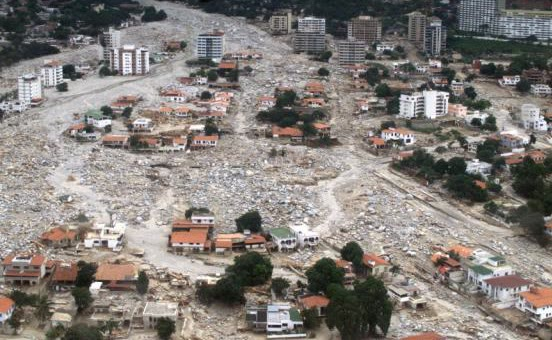
\includegraphics[width=0.62\linewidth]{images/book4/b2-28-caraballeda-debris-flow.jpg}
\par\smallskip{\small Depósitos de \omterm{def:b2:geological-hazards:slope}{flujos de derrubios} en el abanico de Caraballeda, en la costa de Venezuela,
tras la tormenta de diciembre de 1999: los flujos abandonaron el canal principal y sepultaron la ciudad bajo
bloques. Fotografía: Lawson Smith, U.S. Army Corps of Engineers (dominio público).}
\end{omfigure}
% ledger: photo:b2-28-caraballeda, vargas:caraballeda

\section{Los tsunamis}\label{sec:b2:geological-hazards:tsunamis}

Un tsunami generado por el levantamiento repentino del fondo marino tiene una longitud de onda de decenas a cientos de
kilómetros, mucho mayor que la profundidad del océano. Es una onda larga, y su velocidad solo depende
de la profundidad.

\begin{proposition}[Ondas largas]\label{prop:b2:geological-hazards:long-waves}
Una onda de gravedad superficial cuya longitud de onda es mucho mayor que la profundidad del agua $h$ se propaga a
$c = \sqrt{gh}$, sea cual sea su longitud de onda. Donde avanza despacio hacia aguas menos profundas sin
reflejarse ni romper, su amplitud $A$ crece como $h^{-1/4}$.
\end{proposition}

\begin{proof}
La relación de dispersión da la velocidad de fase $c = \omega/k = \sqrt{(g/k)\tanh(kh)}$. Para una onda
larga, $kh = 2\pi h/\lambda \ll 1$, y $\tanh(kh) \approx kh$, así que $c = \sqrt{gh}$, independiente de
$k$: las ondas largas no se dispersan. La energía de la onda por unidad de superficie del mar es $\frac12
\rho g A^2$, y viaja a $c$. Si no se refleja ni se pierde energía, el flujo $\frac12\rho g A^2
c$ a través de cualquier sección es el mismo a lo largo del recorrido: $A^2 \sqrt{h}$ es constante, y $A \propto
h^{-1/4}$.
\end{proof}

Sobre \qty{4000}{m} de agua, un tsunami viaja a \qty{198}{m.s^{-1}}, \qty{713}{km/h}; sobre
\qty{5000}{m}, a \qty{797}{km/h}, los «más de 800 km/h» que citan los servicios de alerta. Cerca de la
costa, en \qty{10}{m} de agua, se frena hasta \qty{36}{km/h}; el agua que viene detrás alcanza su frente,
la onda se acorta y se empina, y su altura crece.
% ledger: nws:tsunami-speed

\begin{definition}[Remonte de un tsunami]\label{def:b2:geological-hazards:tsunami}
El \emph{remonte de un tsunami}\index{remonte de un tsunami} en un punto de la costa es la altura, sobre el
nivel del mar en ese momento, del terreno más alto que el agua alcanza tierra adentro allí. La distancia
horizontal desde la línea de costa hasta ese punto es la distancia de inundación.
\end{definition}

Los equipos de campo miden los remontes a partir de las marcas del agua, las líneas de restos y los daños tras cada tsunami. La
base de datos mundial de tsunamis contiene \num{2177} observaciones de remonte del tsunami del océano Índico del
26 de diciembre de 2004, generado por un terremoto de magnitud 9.1 frente a Sumatra, con una altura máxima del agua de
\qty{50.9}{m}, y \num{6429} del tsunami del 11 de marzo de 2011 frente a Honshu, también de magnitud 9.1,
con un máximo de \qty{39.3}{m}. Los dos mataron a \num{227899} y \num{18423} personas. En Banda Aceh,
el agua llegó a la mitad del segundo piso de la mezquita que se ve abajo.
% ledger: ncei:tsu-2004, ncei:tsu-2011, usgs:aceh-mosque

\begin{omfigure}
\centering
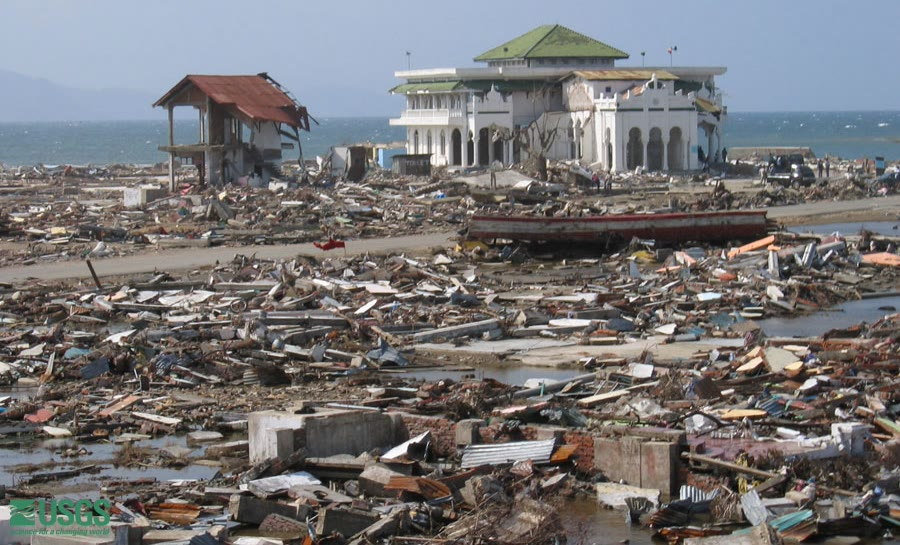
\includegraphics[width=0.62\linewidth]{images/book4/b2-28-aceh-mosque-tsunami.jpg}
\par\smallskip{\small Banda Aceh, Sumatra, el 21 de enero de 2005, tras el tsunami del 26 de diciembre
de 2004: una mezquita sigue en pie entre los escombros de los edificios que la rodeaban. Fotografía: U.S. Geological
Survey (dominio público).}
\end{omfigure}
% ledger: photo:b2-28-aceh

\section{Las crecidas}\label{sec:b2:geological-hazards:floods}

\begin{definition}[Curva de frecuencia de crecidas]\label{def:b2:geological-hazards:flood}
La \emph{curva de frecuencia de crecidas}\index{curva de frecuencia de crecidas} de un río en una estación de aforo es la
curva del caudal máximo anual frente a su \omterm{def:b2:geological-hazards:return}{periodo de retorno}, o a su probabilidad anual de excedencia,
construida a partir del registro de caudales máximos anuales de la estación y extendida habitualmente mediante una ley de
probabilidad ajustada.
\end{definition}

La fórmula del rango de los volúmenes escolares sitúa los puntos de la curva. Tiene una razón de ser.

\begin{proposition}[Posición de trazado de Weibull]\label{prop:b2:geological-hazards:weibull}
Sean $n$ caudales máximos anuales independientes y extraídos de una misma distribución continua, y sea
$G(x)$ la probabilidad de que el máximo de un año supere $x$. El máximo de rango $m$, contado desde el
mayor, tiene una \omterm{def:b2:geological-hazards:poisson}{probabilidad de excedencia} esperada $m/(n + 1)$, de modo que se representa en $T = (n +
1)/m$.
\end{proposition}

\begin{proof}
$U = G(X)$ es uniforme en $[0, 1]$ para una ley continua, y $G$ es decreciente, así que el
$m$-ésimo máximo más grande corresponde a la $m$-ésima más pequeña de $n$ variables uniformes independientes,
$U_{(m)}$. Su densidad es $f(u) = \frac{n!}{(m-1)!\,(n-m)!}u^{m-1}(1-u)^{n-m}$: uno de los $n$ valores
en $u$, $m - 1$ por debajo y $n - m$ por encima. Con la integral Beta $\int_0^1 u^{p}(1-u)^{q}\,\mathrm{d}u
= p!\,q!/(p + q + 1)!$,
\begin{equation*}
\mathbb{E}[U_{(m)}] = \frac{n!}{(m-1)!\,(n-m)!}\cdot\frac{m!\,(n-m)!}{(n+1)!} = \frac{m}{n+1}. \qedhere
\end{equation*}
\end{proof}

El mayor máximo de un registro de 30 años se representa así en 31 años, y nada en el registro fija
la crecida de 100 años. Para alcanzarla, los máximos se ajustan con una ley de extremos, a menudo la de Gumbel,
$\Pr(\text{máximo} \leq x) = \exp\bigl(-e^{-(x - u)/\alpha}\bigr)$, cuya crecida de $T$ años es $x_T = u
- \alpha\ln\bigl(-\ln(1 - 1/T)\bigr)$: una recta frente a $-\ln(-\ln(1 - 1/T))$, extrapolada
más allá del registro con un riesgo que crece con la distancia.

\section{Vigilancia y alerta temprana}\label{sec:b2:geological-hazards:warning}

\begin{definition}[Sistema de alerta temprana]\label{def:b2:geological-hazards:warning}
Un \emph{sistema de alerta temprana}\index{sistema de alerta temprana} es un sistema integrado de vigilancia del
peligro, previsión, evaluación del riesgo, comunicación y preparación que permite actuar a tiempo
antes de un suceso peligroso. Reúne cuatro elementos: el conocimiento del riesgo; la detección,
la vigilancia y la previsión del peligro; la difusión de las alertas; y la preparación para
responder.
\end{definition}
% ledger: undrr:ews

La física fija cuánto tiempo puede dar cada alerta. Es imposible adelantarse a las ondas sísmicas, pero las ondas S,
las que causan daños, viajan a unos \qty{3.2}{km.s^{-1}} en la corteza superior, frente a \qty{5.8}{km.s^{-1}} de
las ondas P: una alerta calculada a partir de las primeras ondas P registradas cerca del epicentro llega a una ciudad
antes que las ondas S, con $d(1/3.2 - 1/5.8) = \qty{0.14}{s}$ por kilómetro de distancia $d$, menos el
tiempo de detección y de cálculo. Una ciudad a \qty{100}{km} gana como mucho \qty{14}{s}; cerca de la fuente, una
zona ciega no recibe ninguno (\cref{exo:b2:geological-hazards:12}). Un tsunami que cruza \qty{100}{km} de mar
de \qty{2000}{m} de profundidad tarda 12 minutos; a través de un océano tarda horas. En 2011, la alerta japonesa
se emitió unos tres minutos después del terremoto, pero con una magnitud estimada demasiado baja,
porque los instrumentos se saturaron; se actualizó con los datos de una boya GPS mar adentro unos 28 minutos después.
Unos registradores de presión de mar profundo, que convierten la presión sobre el fondo marino cada 15 segundos en una
altura de la superficie del mar, informan hoy por satélite del paso de los tsunamis.
% ledger: data:prem, jma:warning, ndbc:dart
% values: 0.1401 s/km, 14.0 s at 100 km; 140 m/s over 2000 m, 11.9 min per 100 km (calc/ch28.py)

\begin{inthefield}[Vigilar un talud que se mueve]
En un talud conocido por su reptación, los equipos de vigilancia instalan instrumentos que miden las variables de la
ecuación del talud infinito. Los piezómetros en sondeos registran la presión intersticial sobre la superficie de deslizamiento;
los tubos inclinométricos, leídos a intervalos de profundidad, muestran dónde se curva el terreno y a qué velocidad; las estaciones
GNSS y los extensómetros registran el movimiento de la superficie; un pluviómetro registra el desencadenante.
Los equipos comparan el movimiento con la lluvia y la presión del agua, estación tras estación, y buscan
la aceleración que precede a la rotura.
\end{inthefield}

\section*{Ejercicios}\label{sec:b2:geological-hazards:exercises}

Datos de los ejercicios, salvo aviso contrario: $g = \qty{9.81}{m.s^{-2}}$; peso específico del agua
\qty{9.81}{kN.m^{-3}}; la GMPE \eqref{eq:b2:geological-hazards:gmpe} en roca ($G_B = G_C = 0$),
$\sigma = 0.230$; velocidades P y S en la corteza superior, 5.8 y \qty{3.2}{km.s^{-1}}. Redondéese a tres
cifras significativas.
% ledger: bjf93:pga, data:prem

\begin{exercise}[$\star$]\label{exo:b2:geological-hazards:1}
Con el modelo de Poisson: (a) ¿cuál es la probabilidad de al menos una crecida de 100 años en 30 años?
(b) ¿Cuál es la probabilidad de que pase un siglo sin una crecida de 100 años? (c) Hállese el \omterm{def:b2:geological-hazards:return}{periodo de retorno}
del movimiento con una \omterm{def:b2:geological-hazards:poisson}{probabilidad de excedencia} del \qty{5}{\percent} en 50 años.
\end{exercise}

\begin{exercise}[$\star$]\label{exo:b2:geological-hazards:2}
Dos ciudades se enfrentan a sacudidas fuertes. En la ciudad A, se producen con una tasa de una vez cada 200 años y
destruirían el \qty{2}{\percent} de sus 5000 edificios; en la ciudad B, una vez cada 50 años, y destruirían el
\qty{10}{\percent} de sus 800 edificios. (a) Hállese el número esperado de edificios destruidos por
año en cada ciudad. (b) ¿Qué ciudad tiene el mayor riesgo, aunque tenga la menor \omterm{def:b2:geological-hazards:risk}{exposición}? (c)
¿Cuál de los tres factores marca la diferencia?
\end{exercise}

\begin{exercise}[$\star$]\label{exo:b2:geological-hazards:3}
(a) Hállese la velocidad de un tsunami sobre profundidades de 4000, 200 y \qty{10}{m}. (b) ¿Cuánto tarda
en cruzar \qty{1500}{km} de océano de \qty{4000}{m} de profundidad? (c) ¿A qué profundidad viajaría a
\qty{800}{km/h}?
\end{exercise}

\begin{exercise}[$\star$]\label{exo:b2:geological-hazards:4}
Una arena seca y sin cohesión con $\varphi' = \ang{33}$ forma un talud largo. (a) Hállese su \omterm{def:b2:geological-hazards:slope}{factor de
seguridad} a \ang{25}. (b) ¿Cuál es el talud más empinado que puede formar? (c) El talud se satura, con
el nivel freático en la superficie y una filtración paralela a ella, de modo que $r_u = \gamma_w\cos^2\beta/\gamma$
con $\gamma = \qty{20}{kN.m^{-3}}$. Demuéstrese que $F = (1 - \gamma_w/\gamma)\tan\varphi'/\tan\beta$ y
calcúlese a \ang{25}.
\end{exercise}

\begin{exercise}[$\star\star$]\label{exo:b2:geological-hazards:5}
El catálogo mundial contiene 696 terremotos de magnitud igual o superior a 7 en los 50 años 1976--2025, y
el intervalo medio entre ellos es de 26.2 días. (a) Hállese su tasa anual media. (b) Con el modelo de
Poisson, ¿cuál es la probabilidad de que pasen 30 días sin ninguno? Compárese con la fracción observada
de intervalos más largos que 30 días, 0.304. (c) ¿Cuál es la probabilidad de al menos uno en una
semana dada?
\end{exercise}

\begin{exercise}[$\star\star$]\label{exo:b2:geological-hazards:6}
(a) Hállese la PGA mediana de un terremoto de magnitud 6.5 en roca a $d = 0$, 10, 30 y
\qty{100}{km}. (b) ¿Cuál sería a \qty{10}{km} en un emplazamiento de clase C? (c) ¿Entre qué valores
se sitúa la PGA en roca a \qty{10}{km} con una probabilidad de alrededor del \qty{68}{\percent}?
\end{exercise}

\begin{exercise}[$\star\star$]\label{exo:b2:geological-hazards:7}
Los caudales máximos anuales de un río durante 12 años fueron, en \unit{m^3.s^{-1}}: 212, 148, 305, 176, 251, 133, 188,
420, 160, 229, 195, 268. (a) Dense los \omterm{def:b2:geological-hazards:return}{periodos de retorno} de los cuatro mayores. (b) Estímese la crecida de 10
años interpolando linealmente en $\ln T$ entre los dos mayores. (c) ¿Por qué este registro no puede decir
nada fiable sobre la crecida de 100 años?
\end{exercise}

\begin{exercise}[$\star\star$]\label{exo:b2:geological-hazards:8}
En un volcán agitado, el observatorio estima: agitación magmática, 0.6; erupción si es magmática, 0.4;
explosiva si hay erupción, 0.5; un \omterm{def:b2:eruptive-styles:pdc}{flujo piroclástico} que alcanza un valle dado si es explosiva, 0.3. (a) Hállese
la probabilidad de un \omterm{def:b2:eruptive-styles:pdc}{flujo piroclástico} en el valle. (b) Hállese la probabilidad de una erupción, y
la de una erupción sin flujo en el valle. (c) Nuevos datos de deformación elevan la probabilidad de una
erupción, si la agitación es magmática, a 0.7. Actualícese (a).
\end{exercise}

\begin{exercise}[$\star\star$]\label{exo:b2:geological-hazards:9}
Un suelo seco con $c' = \qty{8}{kPa}$, $\varphi' = \ang{30}$ y $\gamma = \qty{19}{kN.m^{-3}}$ descansa sobre
un talud de \ang{35}. (a) Hállese el espesor $z_c$ para el que $F = 1$. (b) Hállese $F$ para una capa de
\qty{2}{m} de espesor. (c) La misma capa se satura, con el nivel freático en la superficie y
$r_u = \gamma_w\cos^2\beta/\gamma$. Hállese $F$.
\end{exercise}

\begin{exercise}[$\star\star\star$]\label{exo:b2:geological-hazards:10}
(a) Demuéstrese que el modelo de Poisson no tiene memoria: la probabilidad de ningún suceso en $[s, s + t]$, sabiendo que
no hubo ninguno en $[0, s]$, es $e^{-t/T}$, sea cual sea $s$. (b) Una falla tiene un \omterm{def:b2:geological-hazards:return}{periodo de retorno} de 475 años para sus
grandes terremotos y no ha tenido ninguno en 400 años. ¿Cuál es, según el modelo, la probabilidad de uno
en los próximos 50 años? (c) El rebote elástico del volumen de primer año sugiere que la probabilidad
debería crecer, en cambio, con el tiempo transcurrido desde el último terremoto. ¿Qué hipótesis del modelo de Poisson
contradice, y por qué los mapas de peligrosidad conservan el modelo para las fuentes zonales?
\end{exercise}

\begin{exercise}[$\star\star\star$]\label{exo:b2:geological-hazards:11}
Un tsunami de \qty{0.5}{m} de amplitud y 20 minutos de periodo cruza un océano de \qty{4000}{m} de profundidad. (a)
Con el argumento del flujo de energía de la proposición sobre las ondas largas, hállese su amplitud en \qty{10}{m}
de agua. (b) Hállese su longitud de onda en ambas profundidades. (c) Dense dos razones por las que el remonte en la costa
puede diferir mucho de esta estimación.
\end{exercise}

\begin{exercise}[$\star\star\star$]\label{exo:b2:geological-hazards:12}
Un \omterm{def:b2:geological-hazards:warning}{sistema de alerta temprana} sísmica emite una alerta 4 segundos después de que la onda P llegue a su estación
más cercana al epicentro, a \qty{10}{km}. Despréciese la profundidad de la fuente. (a) ¿Cuándo se
emite la alerta tras el terremoto? (b) ¿Cuántos segundos antes de la onda S la recibe una ciudad a \qty{50}{km}
del epicentro? ¿Y una ciudad a \qty{100}{km}? (c) Hállese el radio de la zona ciega, donde
la onda S llega antes que la alerta.
\end{exercise}

\begin{problem}[{Problema de fin de semana --- Una ciudad entre una falla y un talud}]\label{pb:b2:geological-hazards:1}
Una ciudad sobre roca se encuentra a \qty{10}{km} de una zona sismogénica; todos sus terremotos se toman a
$d = \qty{10}{km}$. Su recurrencia es $\log_{10} N(\geq M) = 4.0 - 1.0\,M$ por año para $M \geq 5$,
truncada en $M_{\max} = 7.5$. La sacudida sigue la GMPE \eqref{eq:b2:geological-hazards:gmpe}
con $\sigma = 0.230$. Por encima de la ciudad, una capa de suelo de \qty{3}{m} de espesor descansa sobre un talud de \ang{30},
con $\gamma = \qty{19}{kN.m^{-3}}$, $c' = \qty{4}{kPa}$ y $\varphi' = \ang{34}$; el agua tiene un peso
específico de \qty{9.81}{kN.m^{-3}}. Redondéese a tres cifras significativas.

\noindent\textbf{Parte I --- La recurrencia.}
\begin{enumerate}
  \item Hállense las tasas anuales de terremotos de magnitud igual o superior a 5, 6 y 7, sin tener en cuenta la
        truncación.
  \item Dense los \omterm{def:b2:geological-hazards:return}{periodos de retorno} correspondientes.
  \item Con la truncación, hállense la tasa de terremotos por encima de 7.5 y la tasa de los comprendidos entre 7
        y 7.5.
  \item Hállense las tasas de las franjas de magnitud 5--6 y 6--7.
  \item ¿Cuál es la probabilidad de al menos un terremoto de magnitud 6 o más en 50 años?
  \item ¿Y de magnitud 7 o más?
\end{enumerate}

\noindent\textbf{Parte II --- El movimiento del suelo en la ciudad.}
\begin{enumerate}[resume]
  \item Hállense $r$ y el término de distancia $-0.778\log_{10} r$.
  \item Represéntense las tres franjas por las magnitudes 5.5, 6.5 y 7.25. Hállense la mediana de
        $\log_{10}\mathrm{PGA}$ y la PGA mediana de cada una.
  \item Hállese la PGA que una magnitud 6.5 supera con una probabilidad del \qty{16}{\percent}.
  \item ¿Cuál es la probabilidad de que una magnitud 6.5 produzca más de \qty{0.3}{g}?
  \item ¿Cuál es la PGA mediana del mayor terremoto posible?
\end{enumerate}

\noindent\textbf{Parte III --- La curva de peligrosidad.}
\begin{enumerate}[resume]
  \item Hállese la tasa anual de excedencia de \qty{0.2}{g}, sumada sobre las tres franjas.
  \item Lo mismo para \qty{0.3}{g}.
  \item Lo mismo para \qty{0.4}{g}.
  \item ¿Qué tasa anual corresponde a un \qty{10}{\percent} en 50 años?
  \item ¿Entre cuáles de los tres niveles se sitúa esa tasa?
  \item Interpolando linealmente $\ln\lambda$ frente a $\ln a$, hállese la PGA con una
        \omterm{def:b2:geological-hazards:poisson}{probabilidad de excedencia} del \qty{10}{\percent} en 50 años.
  \item ¿Qué franjas contribuyen más a la tasa en \qty{0.3}{g}? Coméntese, usando la respuesta a la
        pregunta~11.
\end{enumerate}

\noindent\textbf{Parte IV --- El talud sobre la ciudad.}
\begin{enumerate}[resume]
  \item Hállese el \omterm{def:b2:geological-hazards:slope}{factor de seguridad} del talud seco.
  \item Hállese ese factor cuando la capa está saturada, con el nivel freático en la superficie ($r_u =
        \gamma_w\cos^2\beta/\gamma$).
  \item ¿Hasta qué fracción del espesor de la capa puede subir el nivel freático antes de que el talud rompa?
  \item En un análisis pseudoestático (admitido), la sacudida añade una fuerza horizontal $kW$. Hállese el
        $k$ crítico del talud seco, para el que $F = 1$.
  \item Tomando $k$ igual a la PGA en unidades de $g$, ¿qué magnitud produce el valor crítico como
        su mediana en la ciudad? Compárese con la respuesta a la pregunta~17.
  \item En resumen: ¿cuál es la \omterm{def:b2:geological-hazards:psha}{aceleración máxima del suelo} con una probabilidad del \qty{10}{\percent} de
        superarse en 50 años en la ciudad?
\end{enumerate}
\end{problem}
